\documentclass{article}

\usepackage{fancyhdr}
\usepackage{extramarks}
\usepackage{amsmath}
\usepackage{amsthm}
\usepackage{amsfonts}
\usepackage{amssymb}
\usepackage{xparse}
\usepackage{tikz}
\usepackage{graphicx}
\usepackage[plain]{algorithm}
\usepackage{algpseudocode}
\usepackage{listings}
\usepackage{hyperref}
\usepackage[per-mode = fraction]{siunitx}
\usepackage{calc}

\usetikzlibrary{automata,positioning}

\hypersetup{
    colorlinks=true,
    linkcolor=blue,
    filecolor=magenta,
    urlcolor=blue,
    }

\urlstyle{same}

%
% Basic Document Settings
%

\topmargin=-0.45in
\evensidemargin=0in
\oddsidemargin=0in
\textwidth=6.5in
\textheight=9.0in
\headsep=0.25in

\linespread{1.1}

\pagestyle{fancy}
\lhead{\hmwkAuthorName}
\chead{\hmwkClass\ (\hmwkClassInstructor,\ \hmwkClassTime): \hmwkTitle}
\rhead{\firstxmark}
\lfoot{\lastxmark}
\cfoot{\thepage}

\renewcommand\headrulewidth{0.4pt}
\renewcommand\footrulewidth{0.4pt}

\setlength\parindent{0pt}
\allowdisplaybreaks
%
% Title Page
%

\title{
	\vspace{2in}
	\textmd{\textbf{\hmwkClass:\ \hmwkTitle}}\\
	\normalsize\vspace{0.1in}\small{Due\ on\ \hmwkDueDate\ at \hmwkDueTime}\\
	\vspace{0.1in}\large{\textit{\hmwkClassInstructor,\ \hmwkClassTime}}
	\vspace{3in}
}
\author{\textbf{\hmwkAuthorName}}
\date{\hmwkCompletionDate}

%
% Create Problem Sections
%

\newcommand{\enterProblemHeader}[1]{
	\nobreak\extramarks{}{Problem #1 continued on next page\ldots}\nobreak{}
	\nobreak\extramarks{Problem #1 (continued)}{Problem #1 continued on next page\ldots}\nobreak{}
}

\newcommand{\exitProblemHeader}[1]{
	\nobreak\extramarks{Problem #1 (continued)}{Problem #1 continued on next page\ldots}\nobreak{}
	\nobreak\extramarks{Problem #1}{}\nobreak{}
}

%
% Homework Problem Environment
%
\NewDocumentEnvironment{hwkProblem}{m m s}{
	\section*{Problem #1: #2}
	\enterProblemHeader{#1}
	\setcounter{partCounter}{1}
}{
	\exitProblemHeader{#1}
	\IfBooleanF{#3} % if star, no new page
		{\newpage}
}

% Alias for the Solution section header
\newcommand{\hwkSol}{\vspace{\baselineskip / 2}\textbf{\Large Solution}\vspace{\baselineskip / 2}}

% Alias for the Solution Part subsection header
\newcounter{partCounter}
\newcommand{\hwkPart}{
	\vspace{\baselineskip / 2}
	\textbf{\large Part \Alph{partCounter}}
	\vspace{\baselineskip / 2}
	\stepcounter{partCounter}
}

%
% Various Helper Commands
%

% Such That
\newcommand{\st}{\text{s.t.}}

% Useful for algorithms
\newcommand{\alg}[1]{\textsc{\bfseries \footnotesize #1}}

% For derivatives
\newcommand{\deriv}[1]{\frac{\mathrm{d}}{\mathrm{d}x} (#1)}

% For partial derivatives
\newcommand{\pderiv}[2]{\frac{\partial}{\partial #1} (#2)}

% Integral dx
\newcommand{\dx}{\mathrm{d}x}
\newcommand{\dy}{\mathrm{d}y}

% Probability commands: Expectation, Variance, Covariance, Bias
\newcommand{\e}[1]{\mathrm{e}#1}
\newcommand{\E}{\mathrm{E}}
\newcommand{\Var}{\mathrm{Var}}
\newcommand{\Cov}{\mathrm{Cov}}
\newcommand{\Bias}{\mathrm{Bias}}

% Defining Units that are not in the SI base
\DeclareSIUnit\bar{bar}
\DeclareSIUnit\ft{ft}
\DeclareSIUnit\dollar{\$}
\DeclareSIUnit\cent{\text{\textcent}}
\DeclareSIUnit\c{\degreeCelsius}

% Code Listing config
\usepackage{xcolor}
\definecolor{codegreen}{rgb}{0,0.6,0}
\definecolor{codegray}{rgb}{0.5,0.5,0.5}
\definecolor{codepurple}{rgb}{0.58,0,0.82}
\definecolor{backcolour}{rgb}{0.95,0.95,0.92}
\lstdefinestyle{overleaf}{
	% backgroundcolor=\color{backcolour},
	commentstyle=\color{codegreen},
	keywordstyle=\color{magenta},
	numberstyle=\tiny\color{codegray},
	stringstyle=\color{codepurple},
	basicstyle=\ttfamily\footnotesize,
	breakatwhitespace=false,
	breaklines=true,
	captionpos=b,
	keepspaces=true,
	numbers=left,
	numbersep=5pt,
	showspaces=false,
	showstringspaces=false,
	showtabs=false,
	tabsize=4
}

\usepackage[latte]{catppuccinpalette}
\lstdefinestyle{catppuccin}{
	breaklines=true,
	keepspaces=true,
	numbers=left,
	numbersep=5pt,
	showspaces=false,
	showstringspaces=false,
	breakatwhitespace=true,
	tabsize=4,
	stringstyle = {\color{CtpGreen}},
	commentstyle={\color{CtpOverlay1}},
	basicstyle = {\small\color{CtpText}\ttfamily},
	keywordstyle = {\color{CtpMauve}},
	keywordstyle = [2]{\color{CtpBlue}},
	keywordstyle = [3]{\color{CtpYellow}},
	keywordstyle = [4]{\color{CtpLavender}},
	keywordstyle = [5]{\color{CtpPeach}},
	keywordstyle = [6]{\color{CtpTeal}}
}

\lstset{style=catppuccin}


%
% Homework Details
%   - Title
%   - Subtitle
%   - Due date
%   - Due time
%   - Course
%   - Section/Time
%   - Instructor
%   - Author
%

\newcommand{\hmwkTitle}{Homework 01}
\newcommand{\hmwkSubTitle}{2BP}
\newcommand{\hmwkDueDate}{February 11th, 2025}
\newcommand{\hmwkDueTime}{11:59 PM}
\newcommand{\hmwkClass}{ENAE 404 - 0101}
\newcommand{\hmwkClassTime}{09:30}
\newcommand{\hmwkClassInstructor}{Dr. Barbee}
\newcommand{\hmwkAuthorName}{\textbf{Vai Srivastava}}
\newcommand{\hmwkCompletionDate}{\today}

\begin{document}

\maketitle

\pagebreak

\begin{hwkProblem}{1}{}

	Considering the orbit of Didymos from HW00:
	\begin{enumerate}
		\item Plot the specific energy of the orbit as a function of time.
		\item Using the subplot function, plot the specific angular momentum magnitude and \( x, y, z \) components as a function of time.
		\item Explain why the previous two plots indicate that your 2BP propogator is working properly.
	\end{enumerate}

	\hwkSol

	\hwkPart

	\begin{figure}[ht]
		\begin{center}
			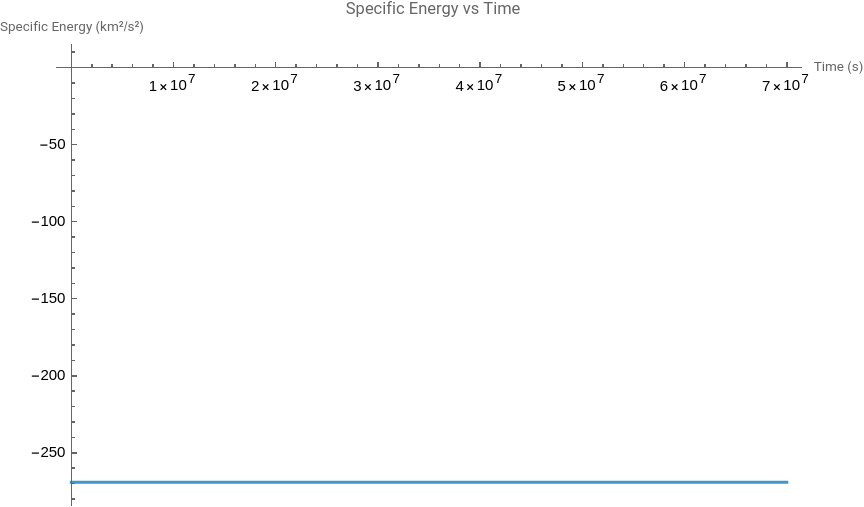
\includegraphics[width=0.95\textwidth]{./images/s01a.png}
		\end{center}
		\caption{Didymos' Specific Energy vs. Time}\label{fig:s01a}
	\end{figure}

	\lstinputlisting[language=mathematica]{./code/s01a.wl}

	\hwkPart

	\begin{figure}[ht]
		\begin{center}
			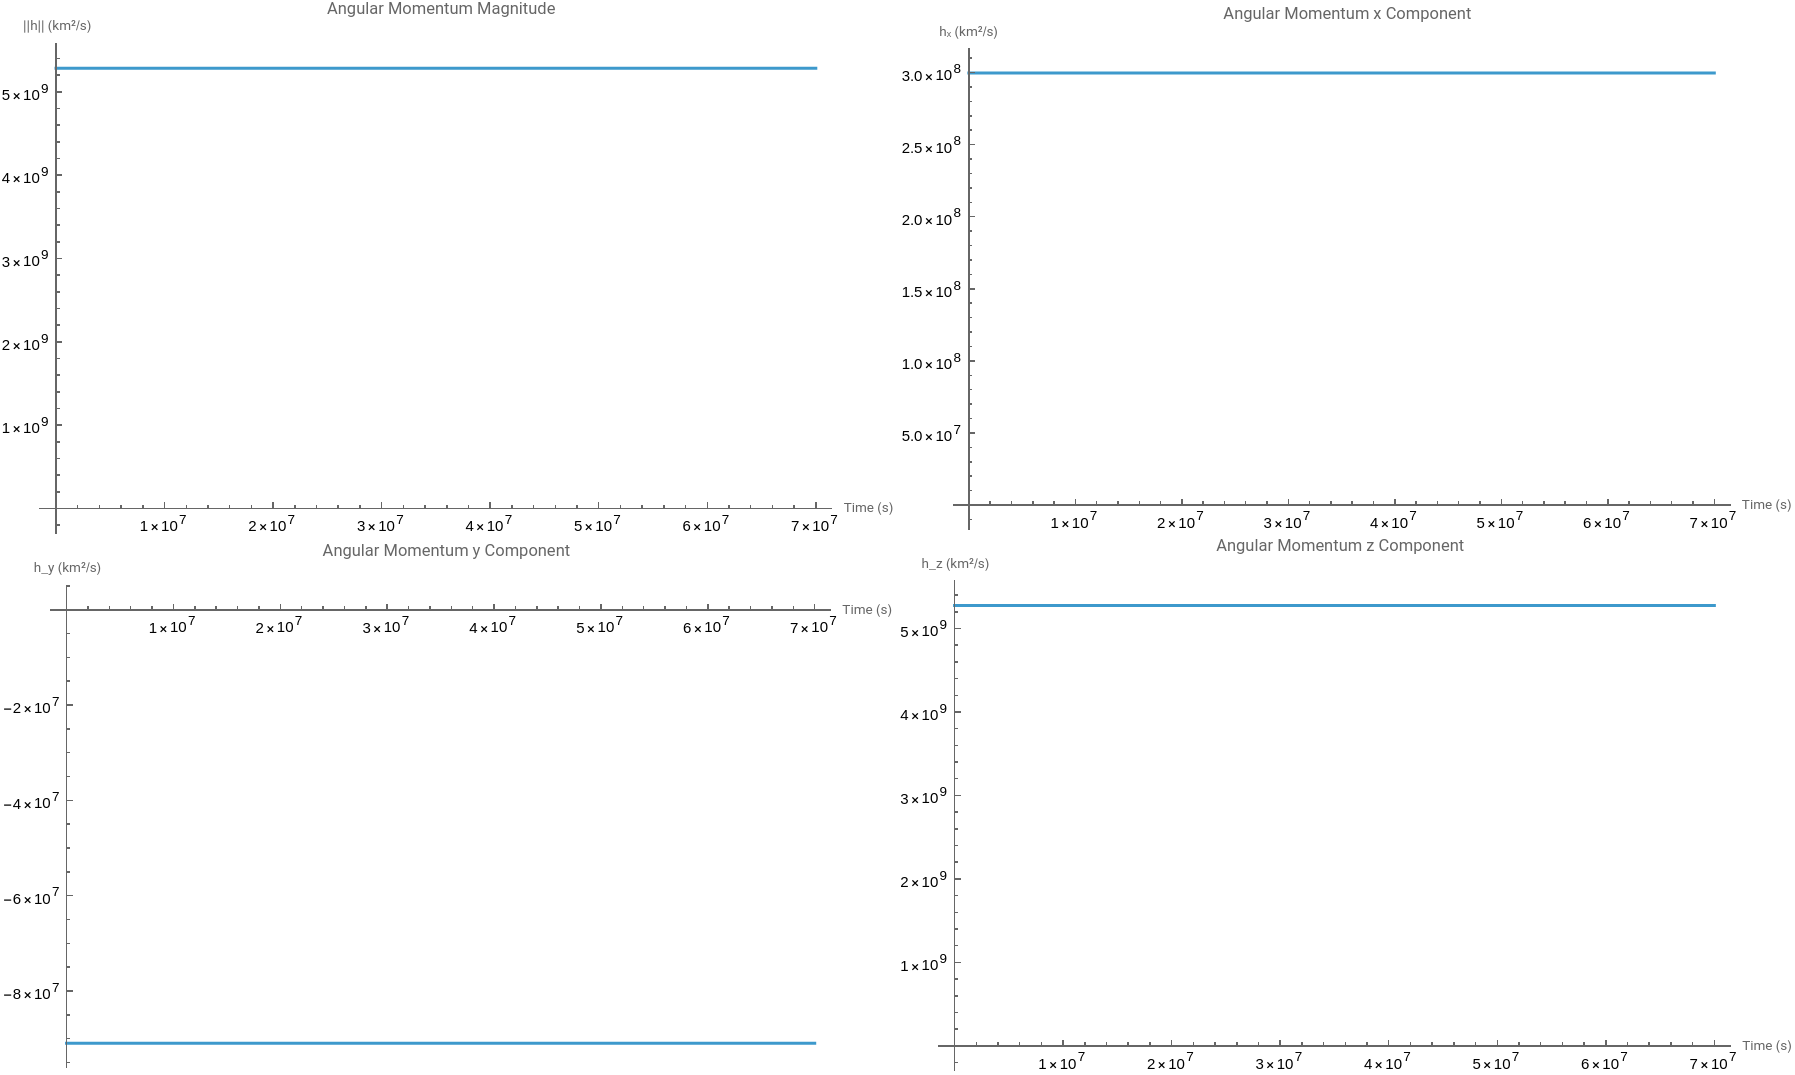
\includegraphics[width=0.95\textwidth]{./images/s01b.png}
		\end{center}
		\caption{Didymos' Components of Specific Angular Momentum vs. Time}\label{fig:s01b}
	\end{figure}

	\lstinputlisting[language=mathematica]{./code/s01b.wl}

\end{hwkProblem}

\begin{hwkProblem}{2}{}
	
	For what value(s) of the true anomaly is the flight path angle zero?
	\begin{enumerate}
		\item For a circle?
		\item For an ellipse?
		\item For a hyperbola?
		\item For a parabola?
	\end{enumerate}
	
	\hwkSol

	\hwkPart

	\[
		\forall \nu \in \mathbb{R} \qed
	\]

	\hwkPart
	\[
		\nu = \qty{0}{\degree}, \qty{180}{\degree} \qed
	\]

	\hwkPart
	\[
		\nu = \qty{0}{\degree} \qed
	\]

	\hwkPart
	\[
		\nu = \qty{0}{\degree} \qed
	\]
	
\end{hwkProblem}

\begin{hwkProblem}{3}{}
	
	The computer in Luke Skywalker's X-Wing is on the fritz. He sees Earth outside his window, and he knows his current altitude is \qty{6e3}{\km}, his velocity is \qty{8.5}{\km\per\s}, and his flight path angle is \qty{0.5}{\degree}. For this problem and all other problems involving Earth orbits in this assignment, use \( \mu = \qty{3.986e5}{\cubic\km\per\square\s} \) and \( \text{Earth Radius} = \qty{6378}{\km} \).
	\begin{enumerate}
		\item What type of conic is Luke's current orbit?
		\item What is the semi-major axis of his orbit?
		\item What is the specific angular momentum magnitude of his orbit?
		\item What is the eccentricity of his orbit?
		\item What is the radius of periapsis of his orbit?
	\end{enumerate}
	
	\hwkSol

	\hwkPart
	\begin{align*}
		\epsilon & = \frac{v^2}{2} - \frac{\mu}{r} \\
		\epsilon & = \qty{3.923}{\kJ\per\kg} \\
		\epsilon & > 0 \qed
	\end{align*}
	\( \therefore \) The orbit is hyperbolic.

	\hwkPart
	\begin{align*}
		\epsilon & = \frac{-\mu}{2a} \implies a = \frac{-\mu}{2\epsilon} \\
		a & = \qty{-50803}{\km} \qed
	\end{align*}

	\hwkPart
	\begin{align*}
		h & = rv\cos{\gamma} \\
		h & = \qty{105209}{\square\km\per\s} \qed
	\end{align*}

	\hwkPart
	\begin{align*}
		p & = a \left( 1 - e^2 \right) = \frac{h^2}{\mu} \\
		\implies e & = \sqrt{1 - \frac{h^2}{a \mu}} \\
		e & = 1.244 \qed
	\end{align*}

	\hwkPart
	\begin{align*}
		r_p & = a \left( 1 - e \right) \\
		r_p & = \qty{12377}{\km} \qed
	\end{align*}
	
\end{hwkProblem}

\begin{hwkProblem}{4}{}
	
	Consider an Earth-orbiting satellite with a semi major axis of \qty{2e4}{\km} and an eccentricity of \( 0.4 \).
	\begin{enumerate}
		\item Calculate the radius of the satellite at a true anomaly of \qty{30}{\degree}.
		\item Calculate the radius of the satellite at a true anomaly of \qty{330}{\degree}.
		\item Calculate the velocity of the satellite at a true anomaly of \qty{30}{\degree}.
		\item Calculate the velocity of the satellite at a true anomaly of \qty{330}{\degree}.
		\item Calculate the flight path angle of the satellite at a true anomaly of \qty{30}{\degree}.
		\item Calculate the flight path angle of the satellite at a true anomaly of \qty{330}{\degree}.
		\item What is the radius of apoapsis of this orbit?
		\item What is the velocity at apoapsis of this orbit?
	\end{enumerate}
	
	\hwkSol

	\hwkPart
	\begin{align*}
		r & = \frac{a \left( 1 - e^2 \right)}{1 + e \cos{\nu}} \\
		r & = \qty{12478}{\km} \qed
	\end{align*}

	\hwkPart
	\begin{align*}
		r \left( \qty{30}{\degree} \right) & = r \left( \qty{330}{\degree} \right) \\
		\implies r & = \qty{12478}{\km} \qed
	\end{align*}
	
	\hwkPart
	\begin{align*}
		v & = \sqrt{\frac{2\mu}{r} - \frac{\mu}{a}} \\
		v & = \qty{6.63}{\km\per\s} \qed
	\end{align*}

	\hwkPart
	\begin{align*}
		r \left( \qty{30}{\degree} \right) & = r \left( \qty{330}{\degree} \right) \\
		\implies v \left( \qty{30}{\degree} \right) & = v \left( \qty{330}{\degree} \right) \\
		\implies v & = \qty{6.63}{\km\per\s} \qed
	\end{align*}

	\hwkPart
	\begin{align*}
		r_p & = a \left( 1 - e \right) \\
		r_p & = \qty{12e3}{\km} \\
		v_p & = \sqrt{\frac{2\mu}{r_p} - \frac{\mu}{a}} \\
		v_p & = \qty{6.819}{\km\per\s} \\
		\gamma & = \arccos{\left(\frac{r_p v_p}{rv}\right)} \\
		\gamma & = \qty{8.43}{\degree} \qed
	\end{align*}

	\hwkPart
	\begin{align*}
		r \left( \qty{30}{\degree} \right) & = r \left( \qty{330}{\degree} \right) \\
		\implies v \left( \qty{30}{\degree} \right) & = v \left( \qty{330}{\degree} \right) \\
		\implies \gamma \left( \qty{30}{\degree} \right) & = \gamma \left( \qty{330}{\degree} \right) \\
		\implies \gamma & = \qty{8.43}{\degree} \qed
	\end{align*}

	\hwkPart
	\begin{align*}
		r_a & = a \left( 1 + e \right) \\
		r_a & = \qty{28e3}{\km} \qed
	\end{align*}

	\hwkPart
	\begin{align*}
		v_a & = \sqrt{\frac{2\mu}{r_a} - \frac{\mu}{a}} \\
		v_a & = \qty{2.923}{\km\per\s} \qed
	\end{align*}
	
\end{hwkProblem}

\begin{hwkProblem}{5}{}
	
	Consider an Earth-centered orbit with a radius of periapsis of \qty{1e4}{\km} and accentricity of \( 1 \).
	\begin{enumerate}
		\item What is the velocity at periapsis?
		\item What is the radius of apoapsis?
		\item What type of conic is this orbit?
	\end{enumerate}
	
	\hwkSol

	\hwkPart
	\begin{align*}
		v_p & = \lim_{a \to \infty} \sqrt{\frac{2\mu}{r_p} - \frac{\mu}{a}} \\
		v_p & = \qty{9.929}{\km\per\s} \\
		v & = \qty{8.929}{\km\per\s} \qed
	\end{align*}

	\hwkPart

	For parabolic orbits, the craft will escape the gravitational pull of the planet, and thus there is neither an apoapsis nor a radius of apoapsis.
	\begin{align*}
		r_a & = \infty \qed
	\end{align*}

	\hwkPart
	\[
		e = 1
	\]
	\( \therefore \) The orbit is parabolic.
	
\end{hwkProblem}

\end{document}
